\documentclass{article}
\usepackage[utf8]{inputenc}
\usepackage{amsmath}
\usepackage{amssymb}
\usepackage{cancel}
\usepackage{graphicx}
\graphicspath{{Images/}}

\setlength{\oddsidemargin}{0in}
\setlength{\textwidth}{6.5in}
\setlength{\topmargin}{-.55in}
\setlength{\textheight}{9in}
\pagestyle{empty}



\title{Problem Set 6 (Astrophysics)}
\author{Michael Nameika}
\date{April 2022}

\begin{document}

\maketitle

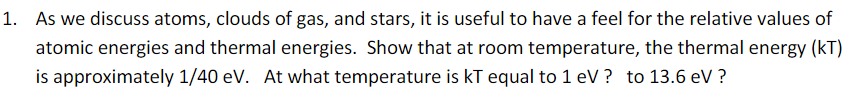
\includegraphics[scale = 0.8]{probset6prob1.PNG}

Using the value of $T = 68^{\circ} F = 293 K$ for room temperature, we find that
\[kT = (8.617 \times 10^{-5} \: \frac{eV}{K})(293 K) \approx 0.0252 eV \approx \frac{1}{40}eV\]
Now we wish to find the temperature when $kT = 1 eV$. That is,
\[T = \frac{1}{K} eV\]
\[ = \frac{1}{8.617 \times 10^{-5} \frac{eV}{K}} eV\]
\[ \approx 11605 K\]
Thus, at a temperature of approximately $11605 K$, $kT = 1 eV$. Now we wish to find the temperature when $kT = 13.6 eV$. Notice if we multiply the previous answer by 13.6, we will find the temperature. Thus,
\[T \approx 157828 K \]
So at a temperature of approximately $157828 K$, $kT = 13.6 eV$
\newline



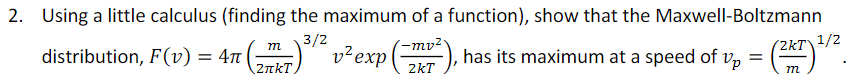
\includegraphics[scale = 0.8]{probset6prob2.PNG}
\newline

We wish to show that $F(v)$ attains its maximum at $v = (\frac{2kT}{m})^{1/2}$. 
Recall that a function attains a minimum or maximum at a critical value, or when that function's first derivative is zero. Notice that
\[F'(v) = 8\pi (\frac{m}{2\pi kT})^{1/2}v\exp{(\frac{-mv^2}{2kT})} - 4\pi(\frac{m}{2\pi kT})^{1/2}v^2(\frac{mv}{kT})\exp{(\frac{-mv^2}{2kT})}\]
And setting $F'(v)$ equal to zero, we find
\[8\pi (\frac{m}{2\pi kT})^{1/2}v\exp{(\frac{-mv^2}{2kT})} - 4\pi(\frac{m}{2\pi kT})^{1/2}v^2(\frac{mv}{kT})\exp{(\frac{-mv^2}{2kT})} = 0\]
\[8\pi (\frac{m}{2\pi kT})^{1/2}v\exp{(\frac{-mv^2}{2kT})} = 4\pi(\frac{m}{2\pi kT})^{1/2}v^2(\frac{mv}{kT})\exp{(\frac{-mv^2}{2kT})}\]
which reduces to
\[2 = v^2(\frac{m}{kT})\]
and clearly,
\[v = (\frac{2kT}{m})^{1/2}\]
which is what we wished to show.
\begin{flushright}
    $\square$
\end{flushright}

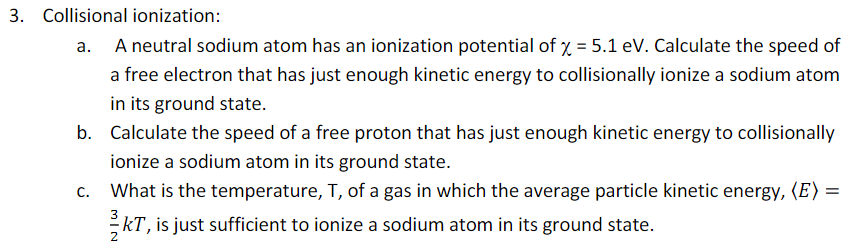
\includegraphics[scale = 0.8]{probset6prob3.PNG}
\newline

a) We are given that $\chi = 5.1 \:eV$, and we wish to find the kinetic energy of a free electron that has just enough kinetic energy to collisionally ionize a sodium atom. That is, if we consider an elastic collision where all of the kinetic energy from the electron is transferred to the sodium atom, we can consider an electron with a kinetic energy of $5.1 \:eV$ and find the speed of said electron.

Ignoring relativistic effects, recall that the classical formula for kinetic energy is given by
\[KE = \frac{1}{2}mv^2\]
and we have that $KE = 5.1 \:eV = 8.175 \times 10^{-19} \:J$, so
\[\frac{1}{2}m_ev_e^2 = 8.175 \times 10^{-19} \:J\]
\[\frac{1}{2}(9.1 \times 10^{-31} \: kg)v_e^2 = 8.175 \times 10^{-19} \:J\]
\[v_e = (\frac{2 \times 8.175 \times 10^{-19} \: J}{9.1 \times 10^{-31} \:kg})^{1/2}\]
\[v_e = 1.34 \times 10^6 \: \frac{m}{s}\]
So a free electron would need to have a minimum kinetic energy of approximately $1.34 \times 10^6 \: \frac{m}{s}$ to ionize a neutral sodium atom.
\newline

b) We wish to find the minimum speed for a free proton to collisionally ionize a neutral sodium atom. Following the same process as above, we find
\[v_p = (\frac{2\times 8.175 \times 10^{-19} \: J}{1.67 \times 10^{-27} \: kg})^{1/2}\]
\[v_p = 3.13 \times 10^4 \: \frac{m}{s}\]
so a free proton would require a speed of approximately $3.13 \times 10^4 \: \frac{m}{s}$ to ionize a neutral sodium atom.
\newline

c) Now we wish to find the temperature of a gas where the average particle kinetic energy is enough to ionize a neutral sodium atom. That is, we want to find the temperature of a gas such that its kinetic energy is at least $5.1 \: eV$.
That is, 
\[\frac{3}{2}(8.617 \times 10^{-5} \frac{eV}{K})T = 5.1 \: eV\]
\[T = \frac{10.2}{3 \times 8.617 \times 10^{-5}}K\]
\[T = 3.95 \times 10^4 \:K\]
So for a gas whose average kinetic energy is given by $<E> = \frac{3}{2}kT$, having a temperature of approximately $3.95 \times 10^4 \:K$ is enough to ionize neutral sodium.
\newline



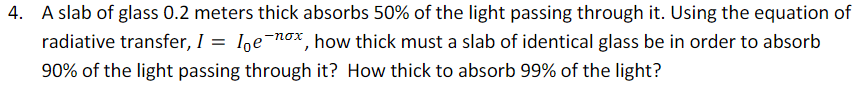
\includegraphics[scale = 0.8]{probset6prob4.PNG}
\newline

We are given that at a thickness of $0.2 \:m$, a slab of glass absorbs 50\% of the light passing through it. We wish to find how thick a slab of identical glass must be to absorb 90\% and 99\% of light. To begin, we know that
\[0.5I_0 = I_0 e^{-n\sigma (0.2) }\]
\[-\ln{(2)} = -n\sigma (0.2)\]
so we have
\[n\sigma = 5\ln{(2)}\]
Now we wish to find the thickness of a slab of glass that absorbs 90\% of the light passing through it. That is, we wish to solve
\[0.1I_0 = I_0e^{-5\ln{(2)}x}\]
for x. Well,
\[-\ln{(10)} = -5\ln{(2)}x\]
\[x = \frac{\ln{(10)}}{5\ln{(2)}}\]
\[x \approx 0.66 \:m\]
That is, a slab of glass approximately $0.66 \:m$ thick will absorb 90\% of light passing through it.

Now we wish to find the thickness of a slab that absorbs 99\% of light passing through it. Similar to the process above, we have
\[0.01I_0 = I_0e^{-5\ln{(2)}x}\]
\[-\ln{(100)} = -5\ln{(2)}x\]
\[x = \frac{\ln{(100)}}{5\ln{(5)}}\]
\[x \approx 1.33 \:m\]
That is, a slab of glass would require a thickness of approximately $1.33 \:m$ to absorb 99\% of the light passing through it.
\newline

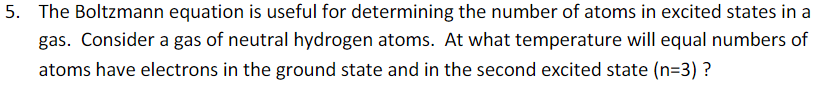
\includegraphics[scale = 0.8]{probset6prob5.PNG}
\newline

To begin, recall the Boltzmann equation:
\[\frac{n_B}{n_A} = \frac{g_B}{g_A}\exp{(\frac{E_A - A_B}{kT})}\]

For neutral hydrogen, we have that $g_n = 2n^2$, and wish to find the temperature when the number of atoms in the ground state ($n = 1$ state) is equal to the number of atoms in the second excited state ($n = 3$ state). Also recall that the energy states of neutral hydrogen are given by $E_n = \frac{-13.6}{n^2} \: eV$.
That is, we wish to find $T$ whenever $\frac{n_3}{n_1} = 1$. 
To begin, let's first find $E_1$ and $E_3$:
\[E_1 = \frac{-13.6}{1^2} \:eV\]
\[ = -13.6 \:eV\]
and $E_3$:
\[E_3 = \frac{-13.6}{3^2} \: eV\]
\[ = -1.51 \: eV\]
Now plugging these values into the Boltzmann equation, we find
\[1 = 9\exp{(\frac{-13.6 \: eV + 1.51 \:eV}{(8.617 \times 10^{-5} \: eV/K)T})}\]
\[\ln{(9)} = \frac{12.09 \: eV}{(8.617 \times 10^{-5} eV/K)T}\]
\[T = \frac{12.09}{(8.617 \times 10^{-5})\ln{(9)}}K\]
\[T \approx\]
 

\end{document}
